% --- Template for thesis / report with tktltiki2 class ---
% 
% last updated 2013/02/15 for tkltiki2 v1.02

\documentclass[finnish,12pt]{tktltiki2}


% tktltiki2 automatically loads babel, so you can simply
% give the language parameter (e.g. finnish, swedish, english, british) as
% a parameter for the class: \documentclass[finnish]{tktltiki2}.
% The information on title and abstract is generated automatically depending on
% the language, see below if you need to change any of these manually.
% 
% Class options:
% - grading                 -- Print labels for grading information on the front page.
% - disablelastpagecounter  -- Disables the automatic generation of page number information
%                              in the abstract. See also \numberofpagesinformation{} command below.
%
% The class also respects the following options of article class:
%   10pt, 11pt, 12pt, final, draft, oneside, twoside,
%   openright, openany, onecolumn, twocolumn, leqno, fleqn
%
% The default font size is 11pt. The paper size used is A4, other sizes are not supported.
%
% rubber: module pdftex

% --- General packages ---

\usepackage[utf8]{inputenc}
\usepackage[T1]{fontenc}
\usepackage{lmodern}
\usepackage{microtype}
\usepackage{amsfonts,amsmath,amssymb,amsthm,booktabs,color,enumitem,graphicx}
\usepackage[pdftex,hidelinks]{hyperref}
\usepackage{setspace}
\usepackage{multicol}

% Automatically set the PDF metadata fields
\makeatletter
\AtBeginDocument{\hypersetup{pdftitle = {\@title}, pdfauthor = {\@author}}}
\makeatother

% --- Language-related settings ---
%
% these should be modified according to your language

% babelbib for non-english bibliography using bibtex
\usepackage[fixlanguage]{babelbib}
\selectbiblanguage{finnish}

% add bibliography to the table of contents
\usepackage[nottoc]{tocbibind}
% tocbibind renames the bibliography, use the following to change it back
\settocbibname{Lähteet}

% --- Theorem environment definitions ---

\newtheorem{lau}{Lause}
\newtheorem{lem}[lau]{Lemma}
\newtheorem{kor}[lau]{Korollaari}

\theoremstyle{definition}
\newtheorem{maar}[lau]{Määritelmä}
\newtheorem{ong}{Ongelma}
\newtheorem{alg}[lau]{Algoritmi}
\newtheorem{esim}[lau]{Esimerkki}

\theoremstyle{remark}
\newtheorem*{huom}{Huomautus}


% --- tktltiki2 options ---
%
% The following commands define the information used to generate title and
% abstract pages. The following entries should be always specified:

\title{Ohjelmistotuotantomenetelmien kehittyminen\newline 1950-luvulta nykypäivään}
\author{Lauri Suomalainen}
\date{\today}
\level{Kandidaatintutkielma}
\abstract{Tiivistelmä}

% The following can be used to specify keywords and classification of the paper:

\keywords{avainsana 1, avainsana 2, avainsana 3}

% classification according to ACM Computing Classification System (http://www.acm.org/about/class/)
% This is probably mostly relevant for computer scientists
% uncomment the following; contents of \classification will be printed under the abstract with a title
% "ACM Computing Classification System (CCS):"
% \classification{}

% If the automatic page number counting is not working as desired in your case,
% uncomment the following to manually set the number of pages displayed in the abstract page:
%
% \numberofpagesinformation{16 sivua + 10 sivua liitteissä}
%
% If you are not a computer scientist, you will want to uncomment the following by hand and specify
% your department, faculty and subject by hand:
%
% \faculty{Matemaattis-luonnontieteellinen}
% \department{Tietojenkäsittelytieteen laitos}
% \subject{Tietojenkäsittelytiede}
%
% If you are not from the University of Helsinki, then you will most likely want to set these also:
%
% \university{Helsingin Yliopisto}
% \universitylong{HELSINGIN YLIOPISTO --- HELSINGFORS UNIVERSITET --- UNIVERSITY OF HELSINKI} % displayed on the top of the abstract page
% \city{Helsinki}
%


\begin{document}



% --- Front matter ---

\frontmatter      % roman page numbering for front matter

\maketitle        % title page
\makeabstract     % abstract page

\tableofcontents  % table of contents

% --- Main matter ---

\mainmatter       % clear page, start arabic page numbering

\section{Johdanto}
\onehalfspacing

Tämä kandidaatintutkielma tarkastelee ohjelmistotuotantomenetelmien kehittymistä ohjelmistokehittämisen alkuajoista nykypäivään ja lähitulevaisuuteen. Se käsittelee erilaisia ohjelmistotuotantomenetelmiä kronologisesti. Jokaisen menetelmän kohdalla pyrin vastaamaan seuraaviin kysymyksiin:

\begin{itemize}
\item Mistä ohjelmistotuotantomenetelmässä on kyse?
\item Miksi sitä käytetään/käytettiin ja mitä hyötyä siitä on/oli?
\item Mitkä olivat sen heikkoudet?
\end{itemize}

Ohjelmistotuotannon eri osa-alueita tarkastellaan tutkielmassa ohjelmistotuotantomenetelmiä määrittävinä piirteinä. Tämä tarkoittaa sitä, että tarkasteltaessa esimerkiksi miten vaatimusmäärittely toteutetaan jossain tietyssä ohjelmistotuotantomenetelmässä, keskitytään prosessin konkreettisen toteutuksen sijasta sen asemaan ja erityispiirteisiin menetelmän kontekstissa.

Ensimmäiset luvut toimivat pohjustuksena tutkielmalle. Luku 2 esittelee lyhyesti keskeisimmät ohjelmistotuotantoon ja tuotantomenetelmiin liittyvät käsitteet ja Luku 3 käsittelee ohjelmistotuotannon alkuaikoja, jolloin tietokoneet itsessään olivat vielä verrattain uusi ilmiö ja suuret ohjelmistot ja niiden tuottaminen oli vähäistä. Alun alkaen laitteiston rajallisuus sitoi myös ohjelmistojen mahdollisuuksia, mutta laitteiston kehittyessä syntyi tarve organisoidummalle ohjelmistojen kehittämiselle.

Luku 4 käsittelee perinteistä ohjelmistotuotantomallia eli niin sanottua "vesiputousmallia". Tarkastelen mallin perusperiaatteita, sen nousemista aikansa keskeisimmäksi ohjelmistotuotantomenetelmäksi, sen onnistumisia ja epäonnistumisia sekä sen heikkouksia ja siihen kohdistettua kritiikkiä.

Luku 5 tarkastelee inkrementaalisia ja iteratiivisia ohjelmistotuotantomenetelmiä sekä prototyyppaamista. Tyyppiesimerkkeinä käsittelen RUP:ia eli Rational Unified Processia sekä spiraalimallia, jota voidaan pitää vesiputousmallin kehittyneempänä versiona.

Luvussa 6 otetaan tarkasteluun ketterät ohjelmistotuotantomenetelmät. Vaikka ketterä ohjelmistokehitys on kattokäsitteenä monelle erilaiselle menetelmälle kuten XP ja Kanban, käsittelen Scrumia tyyppiesimerkkinä, sillä se on kaikista ketteristä menetelmistä suosituin ja tunnetuin.

Viimeisessä luvussa käsittelen lyhyesti yhteenvetona tämän hetken vallitsevia ohjelmistotuotantomenetelmiä. Tarkastelen myös mahdollista lähitulevaisuuden trendejä ja mahdollisuuksia

\section{Peruskäsitteistöä}
Tietojenkäsittelytieteeseen ja ohjelmistotuotantoon liittyy monia alakohtaisia käsitteitä. Kaikkien termien merkitykset eivät ole suoraan johdettavissa itse termistä, sillä osa termistöstä on verrattain vapaita käännöksiä ulkomaisista termeistä ja osa konsepteista on laajoja. Lisäksi joillain termeillä viitataan puhekielessä  vapaammin eri asioihin. Esimerkiksi softwarella voidaan puhekielessä viitata niin yksittäiseen tietokoneohjelmaan kuin laajaan ohjelmistoonkin. Tämän takia lyhyt käsitteenmäärittely tullee tarpeeseen.

Software eli ohjelmisto käsittää tietokoneohjelman tai -ohjelmia sekä kaiken niihin liittyvän informaation ja materiaalin kuten tietokannat ja dokumentaation. \newline Tietokonelaitteisto eli hardware käsittää tietokoneen fyysiset osat kuten prosessorin ja kovalevyn. Laitteistoa tarvitaan ohjelmistojen suorittamiseen, ja laitteisto tarvitsee toimiakseen toimintaohjeet matalan tason tietokoneohjelmina. Käytännössä tietokoneohjelmistot ja -ohjelmat sekä tietokonelaitteisto eivät ole käyttökelpoisia yksinään, vaan kumpaakin tarvitaan toisen järkevään käyttöön.

Termi software engineering, suomeksi ohjelmistotuotanto, alkoi esiintyä kirjallisuudessa 1960-luvun puolivälissä. Termi itsessään on ollut usein keskustelun ja väittelyn kohteena ja ohjelmistotuotannon kuulumista insinööritieteisiin on kyseenalaistettu. \cite{DBLP:reference/se/Grier10,haikala2003ohjelmistotuotanto,mahoney04}
Watts S. Humphrey on määritellyt ohjelmistotuotannon tarkoittavan kurinalaista laadukkaiden ohjelmistojen tuottamista hyödyntäen niin luonnontieteellisiä, matemaattisia kuin insinööritieteidenkin periaatteita ja käytänteitä\cite{Humphrey:1988:SEP:75110.75122}. IEEE Computer Society määrittelee termin viittaavan kurinalaiseen, systemaattiseen ja arvioitavissa olevaan lähestymistapaan ohjelmistojen tuotannossa, käytössä ja ylläpidossa\cite{swebok}. Ilkka Haikala ja Jukka Märijärvi tulkitsevat määrittelyjen tarkoittavan ohjelmistotyötä, jonka tuloksena syntyvät järjestelmät täyttävät käyttäjiensä kohtuulliset toiveet ja odotukset ja tämän lisäksi valmistuvat laadittujen aikataulujen ja kustannusarvioiden puitteissa\cite{haikala2003ohjelmistotuotanto}.

Ohjelmistotuotantoon kuuluvat kaikki ohjelmistotuotantoprosessin osa-alueet. Haikala ja Märijärvi \cite{haikala2003ohjelmistotuotanto} määrittelevät ne seuraavasti:

\begin{description}
\item[Määrittely] sisältää asiakasvaatimusten analyysin ja niistä johdetaan ohjelmistovaatimukset.
\item[Suunnittelu] pitää sisällään ohjelmiston määrittelyssä jäsenneltyjen toiminnallisuuksien ja ominaisuuksien suunnittelun
\item[Toteutus] tarkoittaa ohjelmiston ohjelmointia sekä testauksen toteutusta
\item[Testaus] pyrkii karsimaan ohjelmistosta ohjelmointivirheitä ja muita vikoja. Tyypillisiä testaustapoja ovat yksikkö- ja integraatiotestaus.
\item[Dokumentointi] käsittää ohjelmistoprojektin aikana tuotettavan kirjallisen materiaalin, kuten projektisuunnitelmat, testaussuunnitelmat ja jopa ohjelmakoodin kommentoinnin.
\item[Käyttöönotto] ja \textbf{ylläpito} ovat asiakkaan ongelmien ratkomista, virheiden korjaamista ja tarvittaessa uusien ominaisuuksien lisäämistä.  
\item[Laatujärjestelmällä] ja \textbf{laadunvarmistuksella} on tarkoitus taata, että ohjelmisto täyttää käyttäjän ja asiakkaan toiveet ja odotukset.
\item[Projektinhallinta] on työkalu ohjelmistotuotantoprojektin organisointiin. Suuret ohjelmistoprojektit koostuvat usein useasta rinnakkain tai peräkkäin etenevistä osaprojekteista ja tällöin niiden järjestelmällinen hallinta voi olla keskeistä koko projektin onnistumisen kannalta. 
\item[Tuotteenhallinta:] Usein kaupallisella ohjelmistolla on useita eri konfiguraatioita jolloin se voidaan aina räätälöidä yksilöllisesti kullekin asiakkaalle sopivaksi. Tuotteenhallinnan tarkoitus on varmistaa, että asiakkaalla on tarvitsemansa toimiva versio ohjelmistosta.
\end{description}
Ohjelmistotuotantomenetelmä on koko ohjelmistotuotantoprosessin kattava viitekehys, joka ohjaa prosessin osa-alueitten käytännön toteutusta.

\section{Ohjelmistotuotannon alkutaival}
1940-luvun puolivälistä 1950-luvun lopun ensimmäiset ohjelmoitavat elektronisesti tallentavat tietokoneet olivat nykystandardeilla mitattuna valtavan kokoisia, hitaita ja muistikapasiteetiltaan mitättömiä. Rajoitustensa vuoksi tietokoneohjelmointia pidettiin toissijaisena ja yksinkertaisena toimena verrattuna itse tietokonelaitteiston suunnitteluun ja rakentamiseen. \cite{DBLP:reference/se/Grier10} Lähemmin ohjelmoinnin kanssa työskenteleville alkoi selvitä ohjelmoinnin monimutkaisuus ja ongelmat, kuten rajoitetun muistin hallinta ja ohjelmien välinen interaktio. Tarve järjestelmälliselle ohjelmien tuotannolle oli syntymässä.

Edsger Dijkstran mukaan alkukantaisilla tietokoneilla ohjelmointi nähtiin tapana venyttää tietokonelaitteiston rajoja ja kehittyneempien tietokoneitten uskottiin tekevän ohjelmoinnista lähes triviaalia kun rajoja ei enää tarvitsisi venyttää. \cite{Dijkstra:1979:HP:1241515.1241525} Niin sanottujen kolmannen sukupolven tietokoneiden tultua markkinoille vuosien 1963 ja 1965 välisenä aikana ohjelmoijat löysivät itsensä kuitenkin uusien ongelmien keskeltä, sillä uusi laitteisto oli myös paljon monimutkaisempi kuin aikaisemmat laitteet. Dijkstra itse summaa suurimpien ongelmien johtuneen kuitenkin tietokonelaitteiston tehokkuuden valtavasta tehokkuuden kasvusta: \begin{quote}
Niin kauan kun ei ollut koneita, ohjelmointi ei ollut mikään ongelma; kun meillä oli muutama heikko tietokone, ohjelmointi oli vähäinen ongelma. Nyt kun meillä on giganttisia tietokoneita, on ohjelmoinnista tullut yhtä giganttinen ongelma! \cite{Dijkstra:1979:HP:1241515.1241525}
\end{quote} Tietotekniikkayritysten hankkiessa uutta tehokkaampaa laitteistoa seurasi luonnollisesti paine myös hyödyntää niiden kapasiteettia. Sen lisäksi, että ohjelmoijat joutuivat kohtaamaan haasteita ja toteuttamaan ratkaisuja joita oli aikaisemmin vain spekuloitu \cite{Dijkstra:1979:HP:1241515.1241525}, huomattiin että koulutetusta tietotekniikka-alan työntekijöistä alkoi olla pulaa kysynnän vain kasvaessa. \cite{DBLP:reference/se/Grier10} Ohjelmistoprojektit alkoivat kallistua ja yhä useammin ne ylittivät reilusti budjettinsa ja aikataulunsa mikäli valmistuivat koskaan.\cite{CHAOS1994} Tätä vaihetta tietotekniikan historiassa on myöhemmin kutsuttu nimellä ohjelmistokriisi, software crisis. Dijkstran mukaan ilmiö tunnustettiin avoimesti vuoden 1968 Naton ohjelmistotuotantokonferenssissa Saksan Garmischissa \cite{Dijkstra:1979:HP:1241515.1241525}. Tapahtuma oli merkittävä myös siksi, että termi Software Engineering käytettiin tuolloin ensi kertaa suuressa virallisessa yhteydessä. Tapahtumassa käsiteltyyn myös ohjelmistojen tuotanto ja laaduvalvontasykliä, koodin uusiokäyttöä sekä insinööritieteiden soveltamista ohjelmistojen tuotantoon. \cite{DBLP:reference/se/Grier10}



\section{Perinteiset ohjelmistotuotantomenetelmät}

Perinteisillä ohjelmistotuotantomenetelmillä viitataan suunnitelmavetoisiin tuotantomenetelmiin, joita määrittää projektin alussa suoritettava laaja vaatimusmäärittely ja yksityiskohtainen suunnittelu ja niitä sarjallisesti seuraavat toteutus-, testaus- ja käyttöönottovaiheet. Menetelmien lineaarisen etenemisen ja 'soljumisen' vaiheesta toiseen vuoksi niitä kutsutaan myös kattotermillä 'vesiputousmalli'. Ensimmäisen kerran mallin dokumentoi H.D. Benington vuonna 1956 artikkelissaan \textit{Production of large computer programs}. \cite{Ruparelia:2010:SDL:1764810.1764814, Benington:1987:PLC:41765.41799} Tohtori Winston Royce julkaisi vuonna 1970 paljon keskustelua herättäneen tekstinsä \textit{Managing the Development of Large Software Systems}. Artikkelissa Royce esittelee yksinkertaisen vesiputousmallin, mutta esittää sitä kohtaan kritiikkiä esittäen siitä iteratiivisempia versioita. Siitä huolimatta, että Roycen oma suositus oli tehdä vesiputousmallin vaiheet kahdesti aluksi tuottaen prototyypin ja myöhemmin varsinaisen tuotteen, artikkeliin on viitattu vesiputousmallin keskeisenä hahmotelmana.

\subsection{Vesiputousmallin rakenne}

Vesiputousmalli koostuu toisiaan seuraavista työvaiheista, joista seuraava aloitetaan aina edellisen valmistuttua. Ajalleen tyypillisesti malli muistuttaa insinööritieteiden suunnitteluprosessia, jossa ennen projektin konkreettista toteuttamista tehdään perinpohjaiset suunnitelmat dokumentointeineen. Niin Benningtonin kuin Roycenkin mallin ensimmäiset askeleet liittyvät projektin vaatimusten määrittelyyn ja kartoitukseen. Roycen mallin ensimmäiset askeleet ovat järjestelmävaatimukset ja ohjelmistovaatimukset\cite{Royce1970}. Benington esittää vaiheet vähän laajemmin aloittaen korkeatasoisella ja yleisluontoisella toimintasuunnitelmavaiheella. Vaiheeseen kuuluu asiakasvaatimukset sekä projektin ajalliset ja budjetilliset vaatimukset. Toimintasuunnitelmavaihetta seuraa toiminnalliset määrittelyt ja laitteistospesifikaatiot. \cite{Benington:1987:PLC:41765.41799} Näiden pohjalta määritellään itse ohjelmiston toiminnalliset-, tehokkuus-, käyttö- ja laatuvaatimukset. Royce painotti dokumentaation tärkeyttä projektin onnistumisen kannalta ja alkuvaiheiden valmistuttua tuloksena tulisi olla määrittelydokumentti ja alustava suunnitteludokumentti. Kun vaatimukset on määritelty siirrytään analyysivaiheeseen, jossa selvitetään vaatimusten tekniset yksityiskohdat. Analyysin perusteella suunnitellaan lopulta itse ohjelmiston yksityiskohdat, joihin kuuluvat muun muassa ohjelmiston arkkitehtuuri, rajapinnat, käyttöliittymä ja testaus. Roycen mukaan suunnitteluvaiheen lopuksi dokumentoituna tulisi olla ohjelmiston lopullinen suunnitelma, käyttöliittymäsuunnitelma sekä ohjelmiston testaussuunnitelma. Ohjelmointivaihe toteutetaan suunnitelmien pohjalta ja niitä seuraten. Ohjelmointivaiheen ollessa ohitse siirrytään testausvaiheeseen, jossa ohjelman eri moduulit testataan yhdessä ja erikseen testaussuunnitelman pohjalta. Lopputuotoksena saadaan dokumentti testauksen tuloksista. Viimeinen vaihe on ohjelmiston käyttöönotto ja ylläpito. Tähän vaiheeseen kuuluu mahdollisten käytössä löydettyjen virheiden korjaaminen ja ohjelmiston muuttaminen tai siihen ominaisuuksien lisääminen mikäli tarve sille syntyy.

\begin{figure}[ht!]
\centering
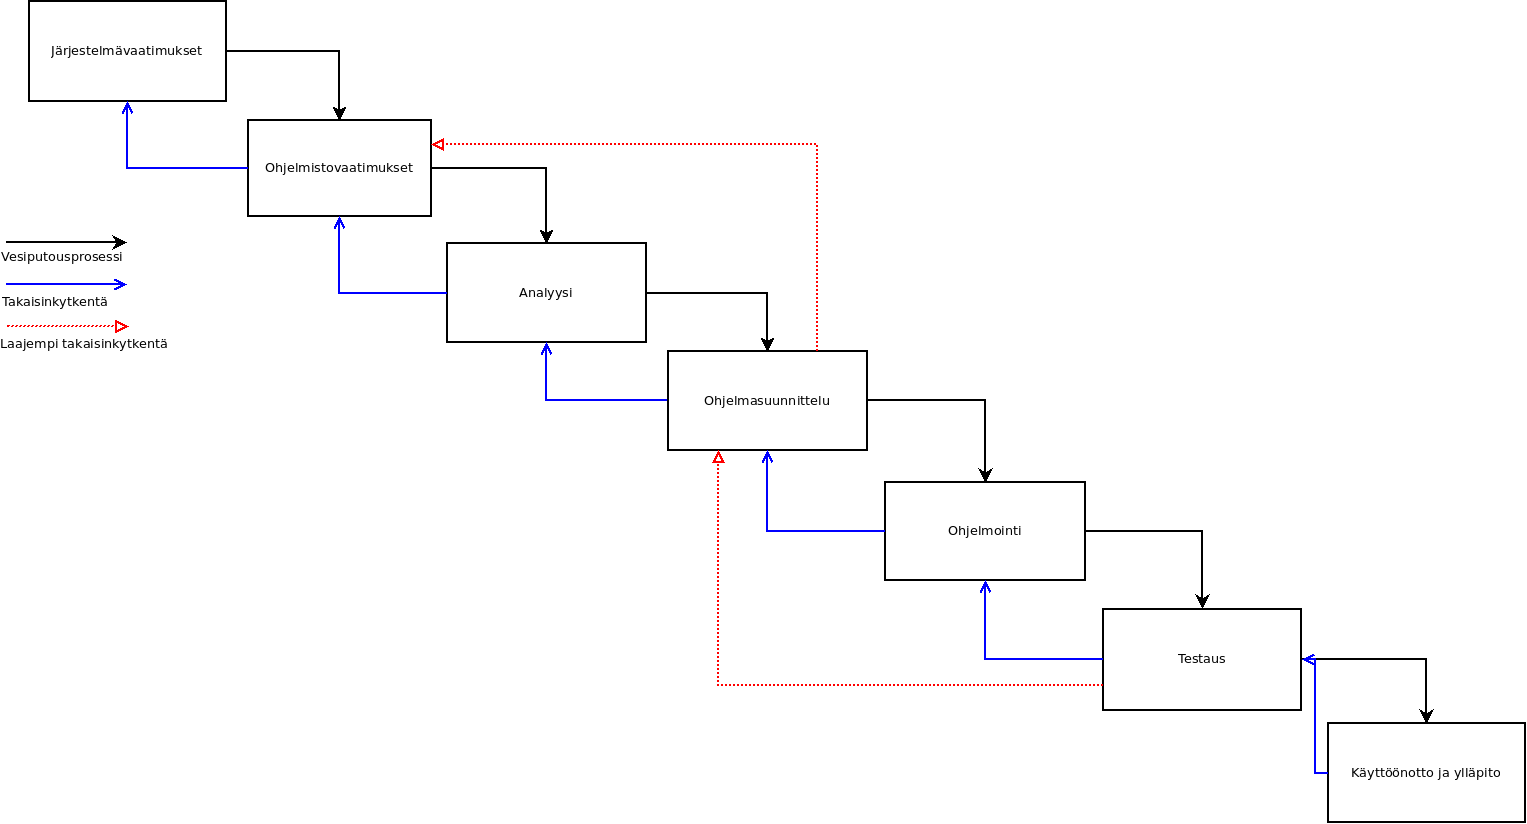
\includegraphics[width=90mm]{Diagram1.png}
\caption{A simple caption}
\label{overflow}
\end{figure}


\subsection{Vesiputousmallin ongelmia}

Koska vesiputousmallille on haettu vaikutteita insinööritieteistä, muistuttaa se paljolti esimerkiksi rakennussuunnitteluprosessia: Siltaa rakentaessa ennen itse rakentamisen aloittamista suunnitellaan sillan arkkitehtuuri, tehdään lujuuslaskelmat, allokoidaan tarvittavat resurssit ja dokumentoidaan suunnitelmat tarkasti. Tarkasti dokumentoiduilla suunnitelmilla itse rakentamisvaihe voitaisiinkin siirtää ulkopuolisen tahon vastuulle ja näin rakennusalalla usein tehdäänkin. \cite{Fowler05} Rakentaminen nähdään triviaalina ja mekaanisena ohjeiden seuraamisena. Martin Fowlerin mukaan menetelmän ongelmana ohjelmistotuotannossa on se, että suunnitelmien virheet ja heikkoudet ilmenevätkin juuri ohjelmointi- ja testausvaiheissa jolloin ohjelmiston toteutus ei olekaan enää kovin suoraviivaista. Juuri suunnittelun korostamisessa piilee myös yksi vesiputousmallin kritisoiduimmista piirteistä. Vesiputousmalli nojaa kokonaisvaltaiseen suunnitteluun ja suunnitelman noudattamiseen, mutta ohjelmistojen kehittäminen tapahtuu usein nopeasti muuttuvassa liiketoimintaympäristössä. Käytännössä on usein mahdotonta selvittää kaiken kattavia ja ulkoisille muutospaineille immuuneja järjestelmä- ja ohjelmistovaatimuksia. \cite{Sommerville10} 

Joskus todelliset vaatimuksetkin selviävät vasta ohjelmistoa oikeassa ympäristössä käytettäessä. Teoriassa hyvä suunnitelma voi osoittautua huonoksi myöhemmissä konkreettemmissa työvaiheissa, mutta vesiputousmallin rakenne vaikeuttaa muutoksien tekemistä suunnitelmiin. Managing the Development of Large Software Systems -artikkelissa Royce esittääkin, että vaiheiden välillä tulisi olla takaisinkytkentöjä, jolloin uutta tietoa saadessa voitaisiin palata korjaamaan aikaisempien työvaiheiden virheitä. \cite{Royce1970} 


\section{Inkremetaaliset ja iteratiiviset menetelmät sekä prototyyppaus}
\section{Ketterät menetelmät}
\section{Ohjelmistojen kehitys nykyään ja tulevaisuudessa}

% --- References ---
%
% bibtex is used to generate the bibliography. The babplain style
% will generate numeric references (e.g. [1]) appropriate for theoretical
% computer science. If you need alphanumeric references (e.g [Tur90]), use
%
% \bibliographystyle{babalpha-lf}
%
% instead.

\bibliographystyle{babplain-lf}
\bibliography{references-fi}


% --- Appendices ---

% uncomment the following

% \newpage
% \appendix
% 
% \section{Esimerkkiliite}

\end{document}
